\documentclass[]{report}
\usepackage[hmargin=1.25in,vmargin=1in]{geometry} %调整页边距
% \usepackage[inner=1in,outer=1.25in]{geometry} %书籍左右不等宽排版
\usepackage[utf8]{inputenc}
\usepackage[]{ctex} %据说可以直接调用诸如 \kaishu \fangsong \heiti 的命令修改字体
\usepackage[svgnames]{xcolor} % Using colors
% \usepackage{background} % To include background images
\usepackage{fancyhdr} % Needed to define custom headers/footers
\usepackage[]{xeCJK}
\setCJKmainfont[BoldFont = STHeiti, ItalicFont = STKaiti]{Songti SC Light} %中文主字体
\setCJKsansfont[BoldFont = Weibei SC, ItalicFont = HanziPen SC]{Xingkai SC Light} %中文无衬线字体
\setCJKmonofont[BoldFont = Libian SC, ItalicFont = STFangsong]{Yuanti SC Light} %中文等宽字体
\setmainfont{Times New Roman} %\rmfamily
\setsansfont[ItalicFont = American Typewriter]{Comic Sans MS} %\sffamily
\setmonofont{Courier} %\ttfamily
\newfontfamily\monaco{Courier} % 用于代码段字体设置
\newfontfamily\OldCaption{Bodoni 72 Smallcaps Book} %用于全大写字母的标题
\usepackage{titlesec}
\titleformat{\chapter}{\centering\huge\bfseries}{第~\thechapter~章}{1em}{}
\titleformat{\section}{\Large\bfseries}{第~\thesection~节}{1em}{}
\usepackage{lipsum} %填充文本

\usepackage{ulem} %解决下划线、删除线之类的
\usepackage{listings}
\lstset{
language=C++,
numberstyle = \monaco,
basicstyle = \monaco,
keywordstyle = \color{blue}\bfseries,
commentstyle=\color[HTML]{006400},
tabsize = 4,
%backgroundcolor=\color{bg}
emph = {int,float,double,char},emphstyle=\color{cyan},
emph = {[2]const, typedef},emphstyle = {[2]\color{red}} }

\makeatletter
\newif\if@restonecol
\makeatother
\let\algorithm\relax
\let\endalgorithm\relax
\usepackage[linesnumbered,ruled,vlined]{algorithm2e}%[ruled,vlined]{
\usepackage{algpseudocode}
\usepackage{amsmath}
\renewcommand{\algorithmicrequire}{\textbf{Input:}}  % Use Input in the format of Algorithm
\renewcommand{\algorithmicensure}{\textbf{Output:}} % Use Output in the format of Algorithm

\usepackage{amsmath} %数学公式问题
\usepackage{amsthm} %公式环境,如proof
\usepackage{booktabs} %三线表
\newcommand{\tabincell}[2]{\begin{tabular}{@{}#1@{}}#2\end{tabular}} %解决单元格内部换行的问题
% 比如这个 Beijing & 0,5 & 1,6 & 2,7 & 3,8 & 4,9 & The number changes every 3 months \\
% 改成这个 \tabincell{l}{Beijing}& \tabincell{c}{0,5}& \tabincell{c}{1,6}& \tabincell{c}{2,7}& \tabincell{c}{3,8}& \tabincell{c}{4,9}& \tabincell{c}{The number changes \\ every 3 months} \\
% 一个单元格过长,整行都需要修改
% 可以配合 \resizebox*{h-width}{v-width}{contents, e.g.tabular} 使用

\usepackage{mathrsfs} %在公式里面使用那个最花的字体
\usepackage{amssymb} %公式里面用空心黑体和旧式字体
\usepackage{amssymb} %AMS符号
\usepackage{amsthm} %AMS定理环境

\usepackage{markdown} %使用markdown语法,在编译时需要打开 shell-escape 标记,即 $ xelatex --shell-escape example.tex
\markdownSetup{hashEnumerators = true} %允许使用 #. 的方式编写有序列表
\markdownSetup{inlineFootnotes = true} %允许使用脚注形式的超链接,调用语法为 [anchor](uri), ^[footnote], <uri>
\markdownSetup{fencedCode = true} %以反引号和缩进来插入代码段,相当于 verbatim
\markdownSetup{
  pipeTables = true
} %支持表格的用法 (图片已经在markdown包里面支持了)
% \usepackage{booktabs} %解决三线表的线条粗细问题

\usepackage{graphicx} %插入图片
\usepackage{pdfpages} %插入PDF文件
\usepackage{makeidx}

\usepackage{tikz} %带圈字符
\usepackage{etoolbox} %带圈字符 (提供robustify)
\usepackage{enumitem}
\newcommand*{\circled}[1]{\lower.7ex\hbox{\tikz\draw (0pt, 0pt)%
    circle (.5em) node {\makebox[1em][c]{\small #1}};}} %新定义命令:带圈字符
\robustify{\circled}
% \usepackage{enumerate} %有序列表

\usepackage{hyperref} %超链接
% \usepackage[hidelinks]{hyperref} %隐藏超链接的红框
\markdownSetup{
  inlineFootnotes = true,
  renderers = {
    link = {\href{#3}{#1}},
  }
} % markdown块中使用直接点进去的超链接
% \setlist[enumerate,1]{label=(\arabic*).,font=\textup,leftmargin=7mm,labelsep=1.5mm,topsep=0mm,itemsep=-0.8mm}
% \setlist[enumerate,2]{label=(\alph*).,font=\textup,leftmargin=7mm,labelsep=1.5mm,topsep=-0.8mm,itemsep=-0.8mm}

\usepackage{braket}

%%%%%% Setting up the style

% \setlength\parindent{0pt} % Gets rid of all indentation
% \backgroundsetup{contents={\includegraphics[width=\textwidth]{ustc-name.pdf}},scale=0.4,placement=top,opacity=0.6,color=cyan,vshift=-20pt} %  USTC Logo

\pagestyle{fancy} % Enables the custom headers/footers

% 使用默认的Chapter页眉
% \lhead{} \rhead{} % Headers - all  empty

% \title{\vspace{-1.8cm}  \color{DarkRed} Laboratory Rotation Report}
% \subtitle{Title of the proposal % Title of the rotation project
% \vspace{-2cm} }
% \date{\today} % No date

\lfoot{\color{Grey} \textit{上官凝}}  % Write your name here
\rfoot{ \color{Grey} 算法基础 }
\cfoot{\color{Grey} \thepage}

\renewcommand{\headrulewidth}{0.0pt} % No header rule
\renewcommand{\footrulewidth}{0.4pt} % Thin footer rule

\title{{\huge {算法基础笔记}}}
\author{上官凝}
\date{\today}

\linespread{1.3} %行间距为1.3倍默认间距 (1.3 x 1.2倍字符宽度)

\makeindex

\begin{document}
\theoremstyle{definition} \newtheorem{theorem}{Thm}[section] %定义一个定理Thm,序号为section的下一级序号
\theoremstyle{definition} \newtheorem{definition}{Def}[section] %定义一个定义Def,序号为section的下一级序号
\theoremstyle{plain} \newtheorem{lemma}{lemma}[section] %引理

	\maketitle
	\newpage

	\tableofcontents
	\newpage

	\chapter{基础知识}
	算法书的\href{https://ita.skanev.com/08/03/02.html}{答案}
	\chapter{以比较为基础的排序算法}
	先引入几个评判标准的概念:
	\begin{enumerate}
		\item 稳定性:(Stability)假定在待排序的记录序列中,存在多个具有相同的关键字的记录,若经过排序,这些记录的相对次序保持不变。\footnote{https://baike.baidu.com/item/排序算法稳定性}
		\item 时间复杂度
		\item 就地排序:只有常数个数的元素被存储在数组外面
	\end{enumerate}
	以下六种方法,前三种(插入排序、选择排序和冒泡排序)是比较基础的排序算法,而后面三种(希尔排序、堆排序和快排)是效率比较高的。
	\section{插入排序}
		插入排序({\OldCaption{Insertion-Sort}})的总体思想是保持一个已经排序完成的DONE序列,类比摸扑克牌并将其顺序置入收卡中
		\begin{algorithm}
			\caption{{\OldCaption{Insertion-Sort}}(A)}
			\ForAll{$j=2$to$A.length$}{
				$key=A[j]$\\
				// Insert $A[j]$ into the sorted sequence $A[1..j − 1]$.\\
				$i=j-1$\\
				\While{$i>0$and$A[i]>key$}{
					$A[i+1]=A[i]$\\
					$i=i-1$
				}
				$A[i+1]=key$
			}
		\end{algorithm}
		时间复杂度:最好$O(n)$,平均和最差都是$O(n^2)$,就地排序,稳定排序
	\section{选择排序}
		与插入排序相反,选择排序({\OldCaption{Selection-Sort}})不再遍历已排序数组,而是遍历未排序数组,选出最小的元素,并将其放入新的数组里面。时间稳定性三个均为$O(n^2)$,是就地排序但不是稳定排序
		\begin{figure}[h!]
			\centering
			\begin{minipage}{40em}
				\centering
				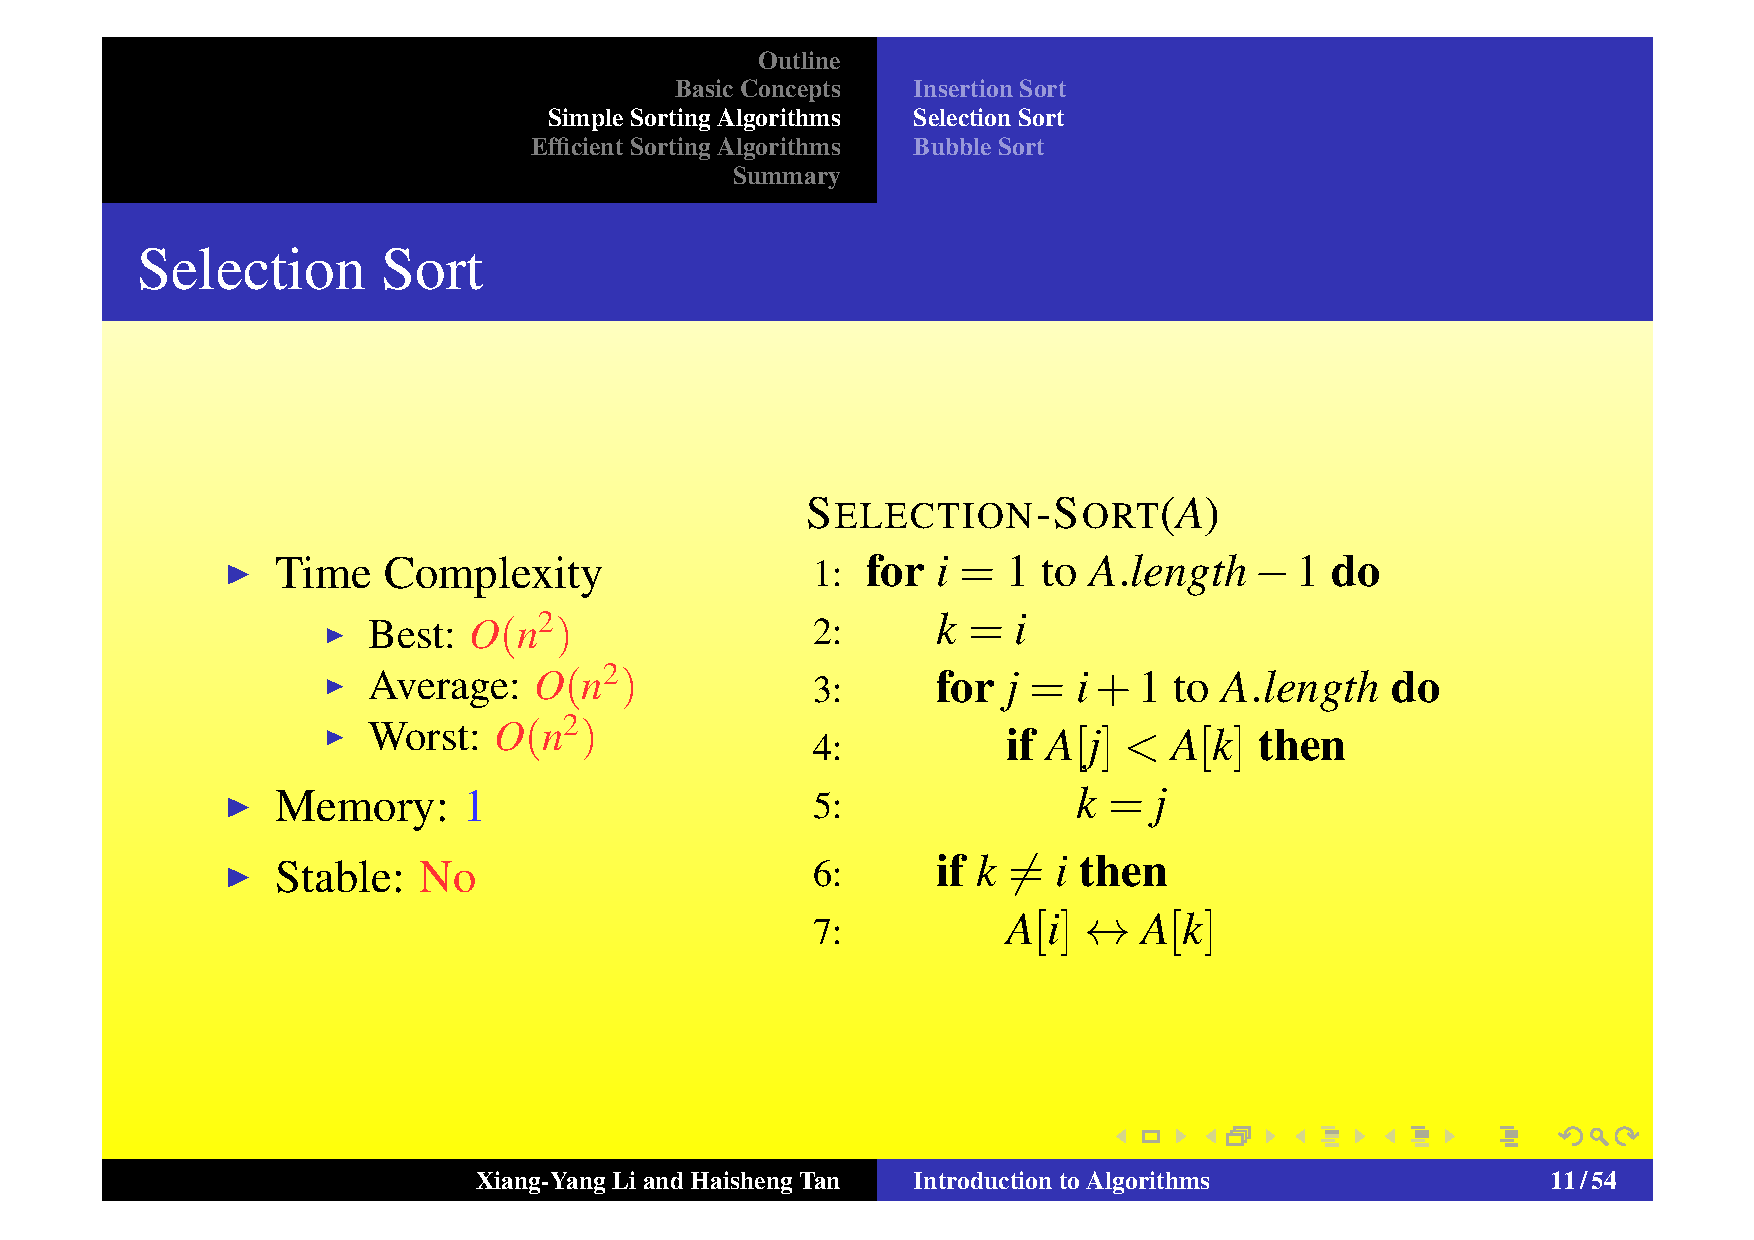
\includegraphics[scale = 0.45]{images/Selection_Sort.pdf}
			\end{minipage}
		\end{figure}
	\section{冒泡排序}
		冒泡排序({\OldCaption{Bubble-Sort}})是两重循环比较相邻两个数据,将较大/小者下沉/上浮
		\begin{figure}[h!]
			\centering
			\begin{minipage}{40em}
				\centering
				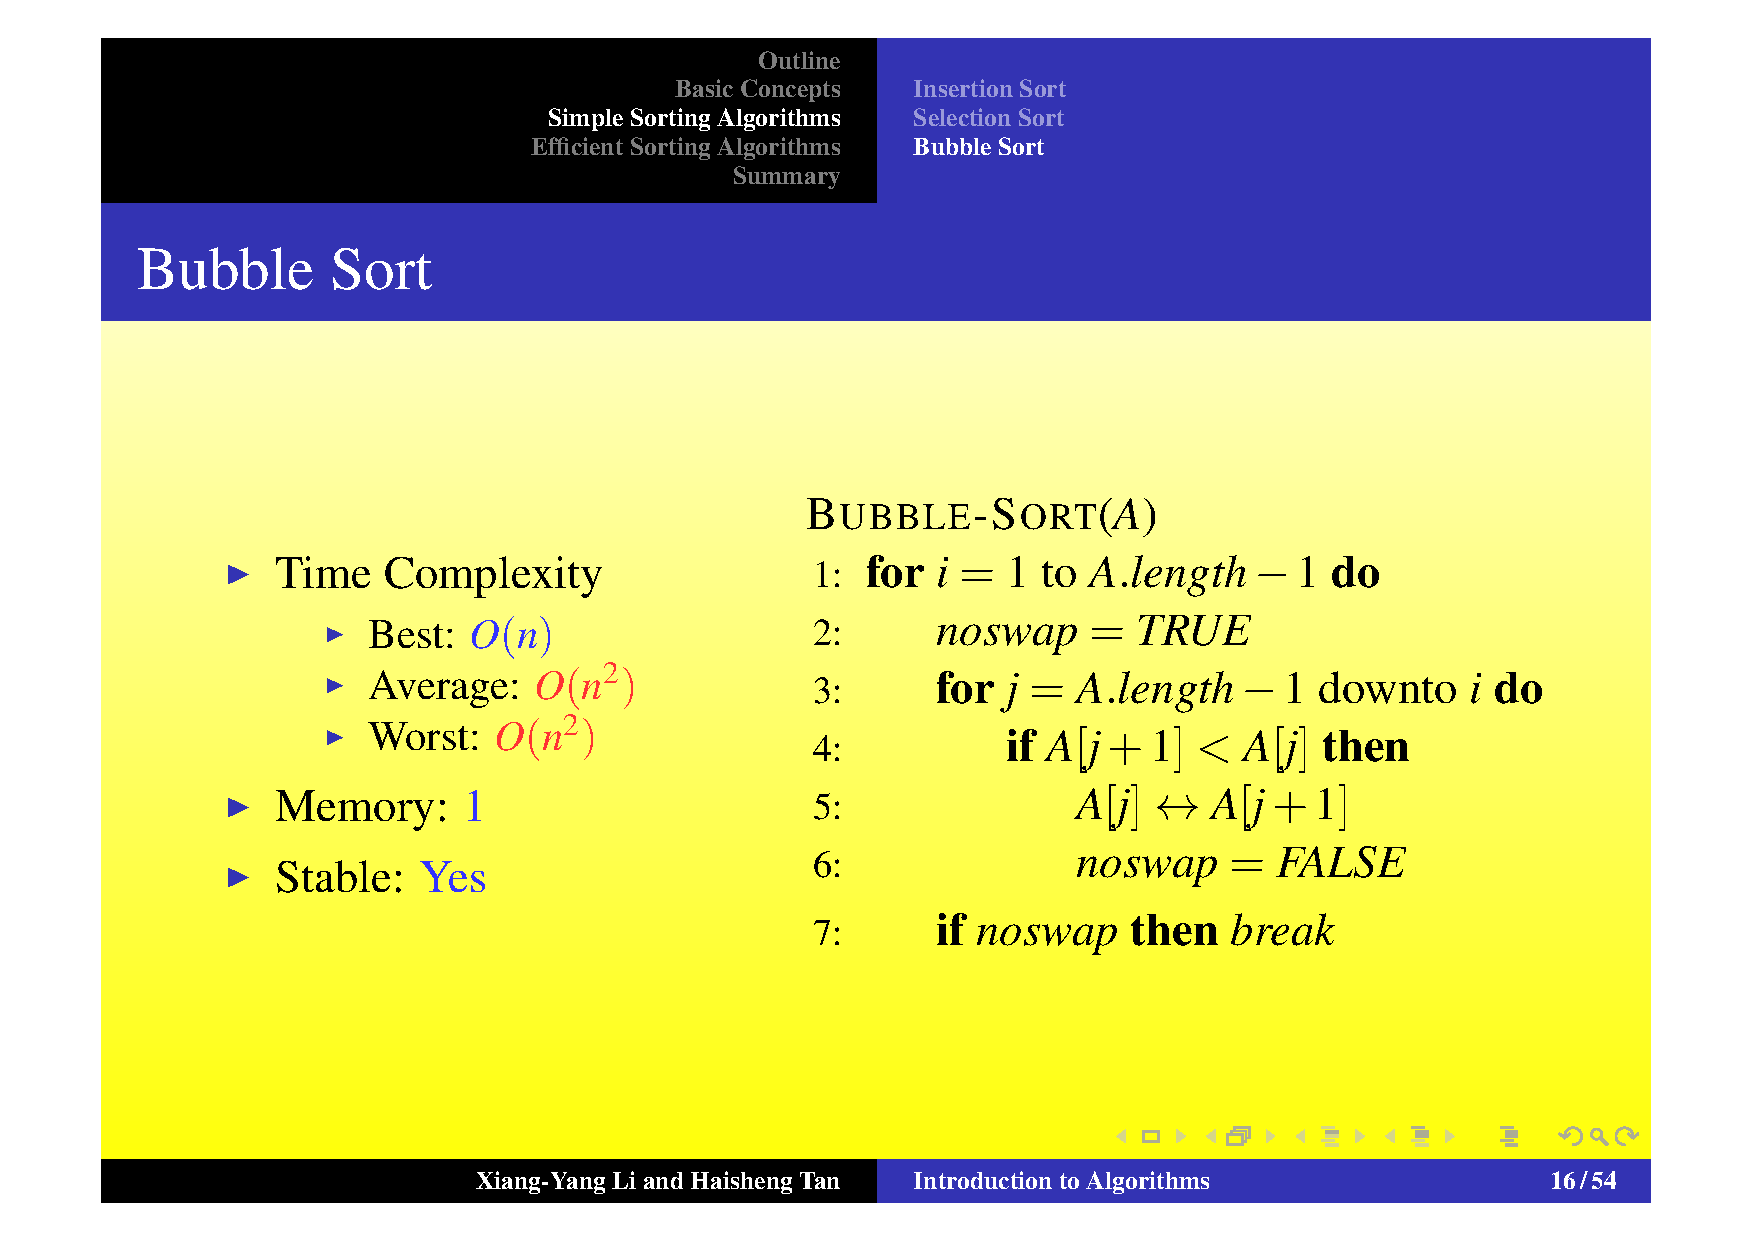
\includegraphics[scale = 0.45]{images/Bubble_Sort.pdf}
			\end{minipage}
		\end{figure}
	\section{希尔排序}
		希尔排序(Shell-Sort)是一种“少吃多餐”的插入排序算法,他需要选取一组递减的\textit{模长},在每一轮排序中,对同一“同余类”中的数据进行插入排序。有一个\href{https://blog.csdn.net/qq_39207948/article/details/80006224}{参考链接}。希尔排序的时间复杂度依赖于间隔序列,属于就地排序,不是稳定排序。\par
		为什么需要用到希尔排序呢?
		\begin{enumerate}
			\item 尽管插入排序的最坏情况时间复杂度是$O(n^2)$,但是在数据总量较小时可以和$O(n)$相接近
			\item 当对一个较大的数组进行排序的时候,如果用一个足够大的排序间隔,每一个sub-array就会比较小
			\item 在很多轮循环之后,尽管gap很小了,但是大部分元素也已经排好序了(所以是一个比较好的情况)
		\end{enumerate}
		那么,如何选择模长呢?
		\begin{enumerate}
			\item $\left\lceil\frac{n}{2^k}\right\rceil$:时间复杂度$\Theta(n^2)$
			\item $2\left\lceil\frac{n}{2^k+1}\right\rceil+1$:时间复杂度$\Theta(n^{3/2})$
			\item $2^k-1$:时间复杂度$\Theta(n^{3/2})$
			\item $2^k+1\ (k\ge0)$:时间复杂度$\Theta(n^{3/2})$
			\item 连续的形如$2^p3^q\ (p,q\mbox{为素数})$的gap:时间复杂度$\Theta(n\lg^2n)$
		\end{enumerate}
	\section{堆排序}
		堆排序({\OldCaption{Heap-Sort}})是一直维护一个二叉堆。然后重复选择排序,只是换做用二叉堆来找到最小/大元素(最大堆的$A[1]$永远是最大的元素。注意到堆有一个很好的性质:with the array representation of an n-element heap, the leaves are the nodes indexed from $\lceil A.length/2\rceil + 1$ to $n$, and each leaf is a 1-element max-heap to begin with.
		\begin{figure}[h!]
			\centering
			\begin{minipage}{20em}
				\centering
				\begin{minipage}{20em}
					\centering
					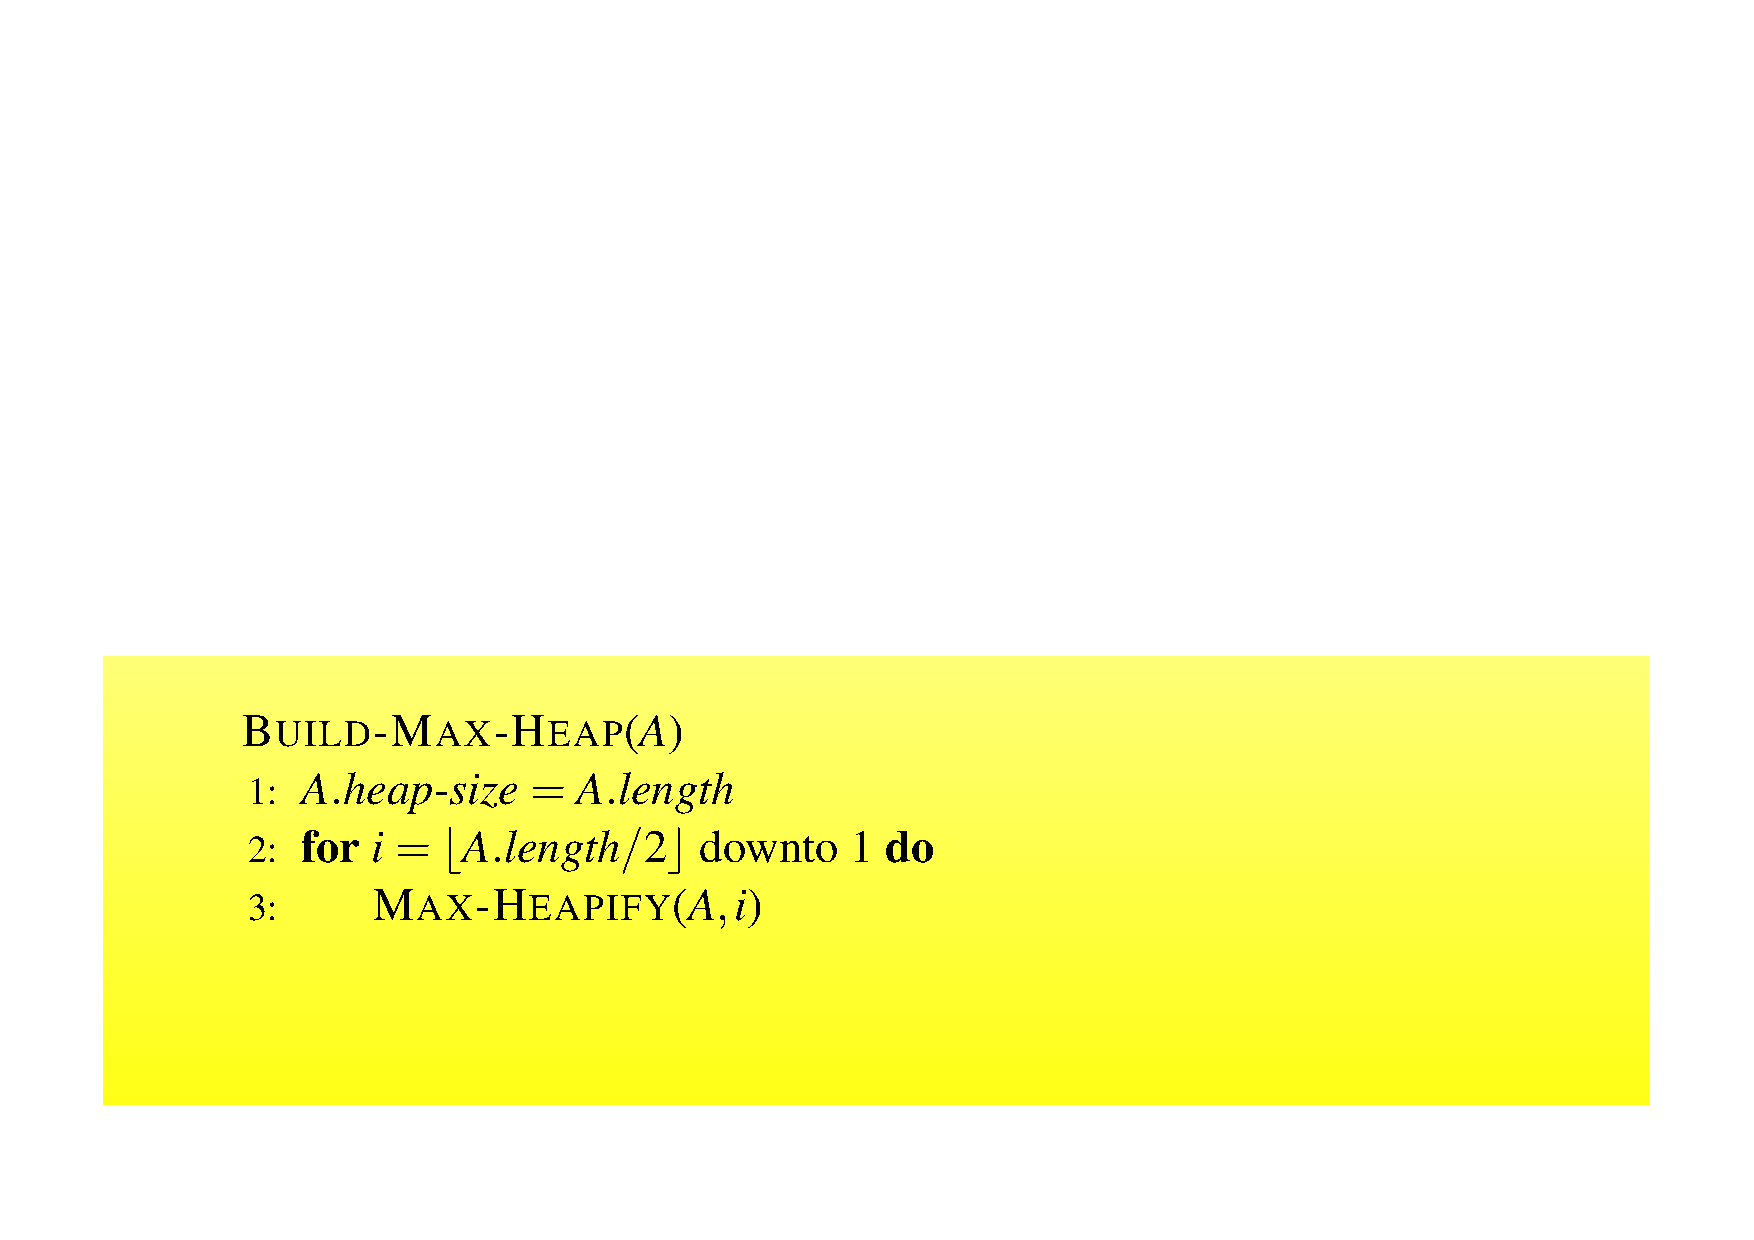
\includegraphics[scale = 0.25]{images/Build_Max_Heap.pdf}
				\end{minipage}\\[10pt]
				\begin{minipage}{20em}
					\centering
					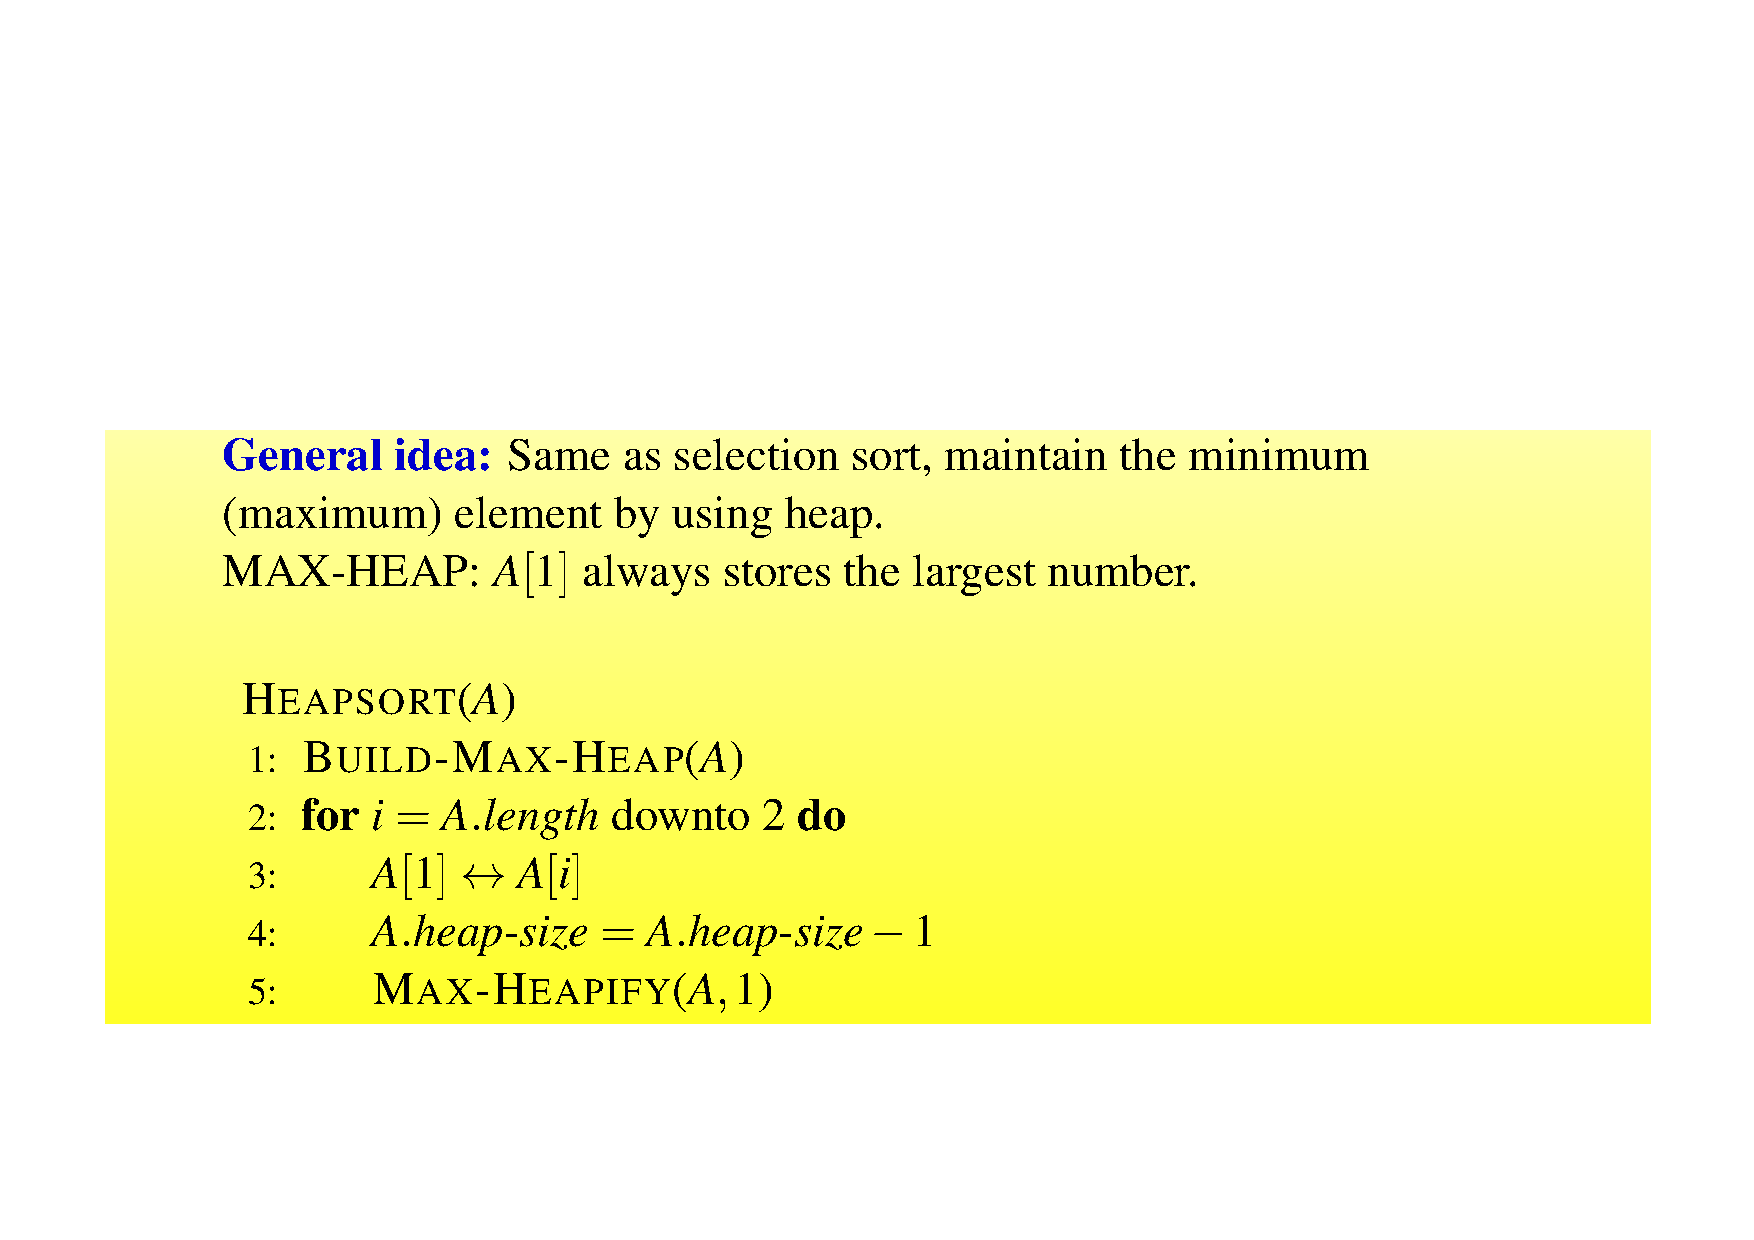
\includegraphics[scale = 0.25]{images/HeapSort.pdf}
				\end{minipage}
			\end{minipage}\quad
			\begin{minipage}{20em}
				\centering
				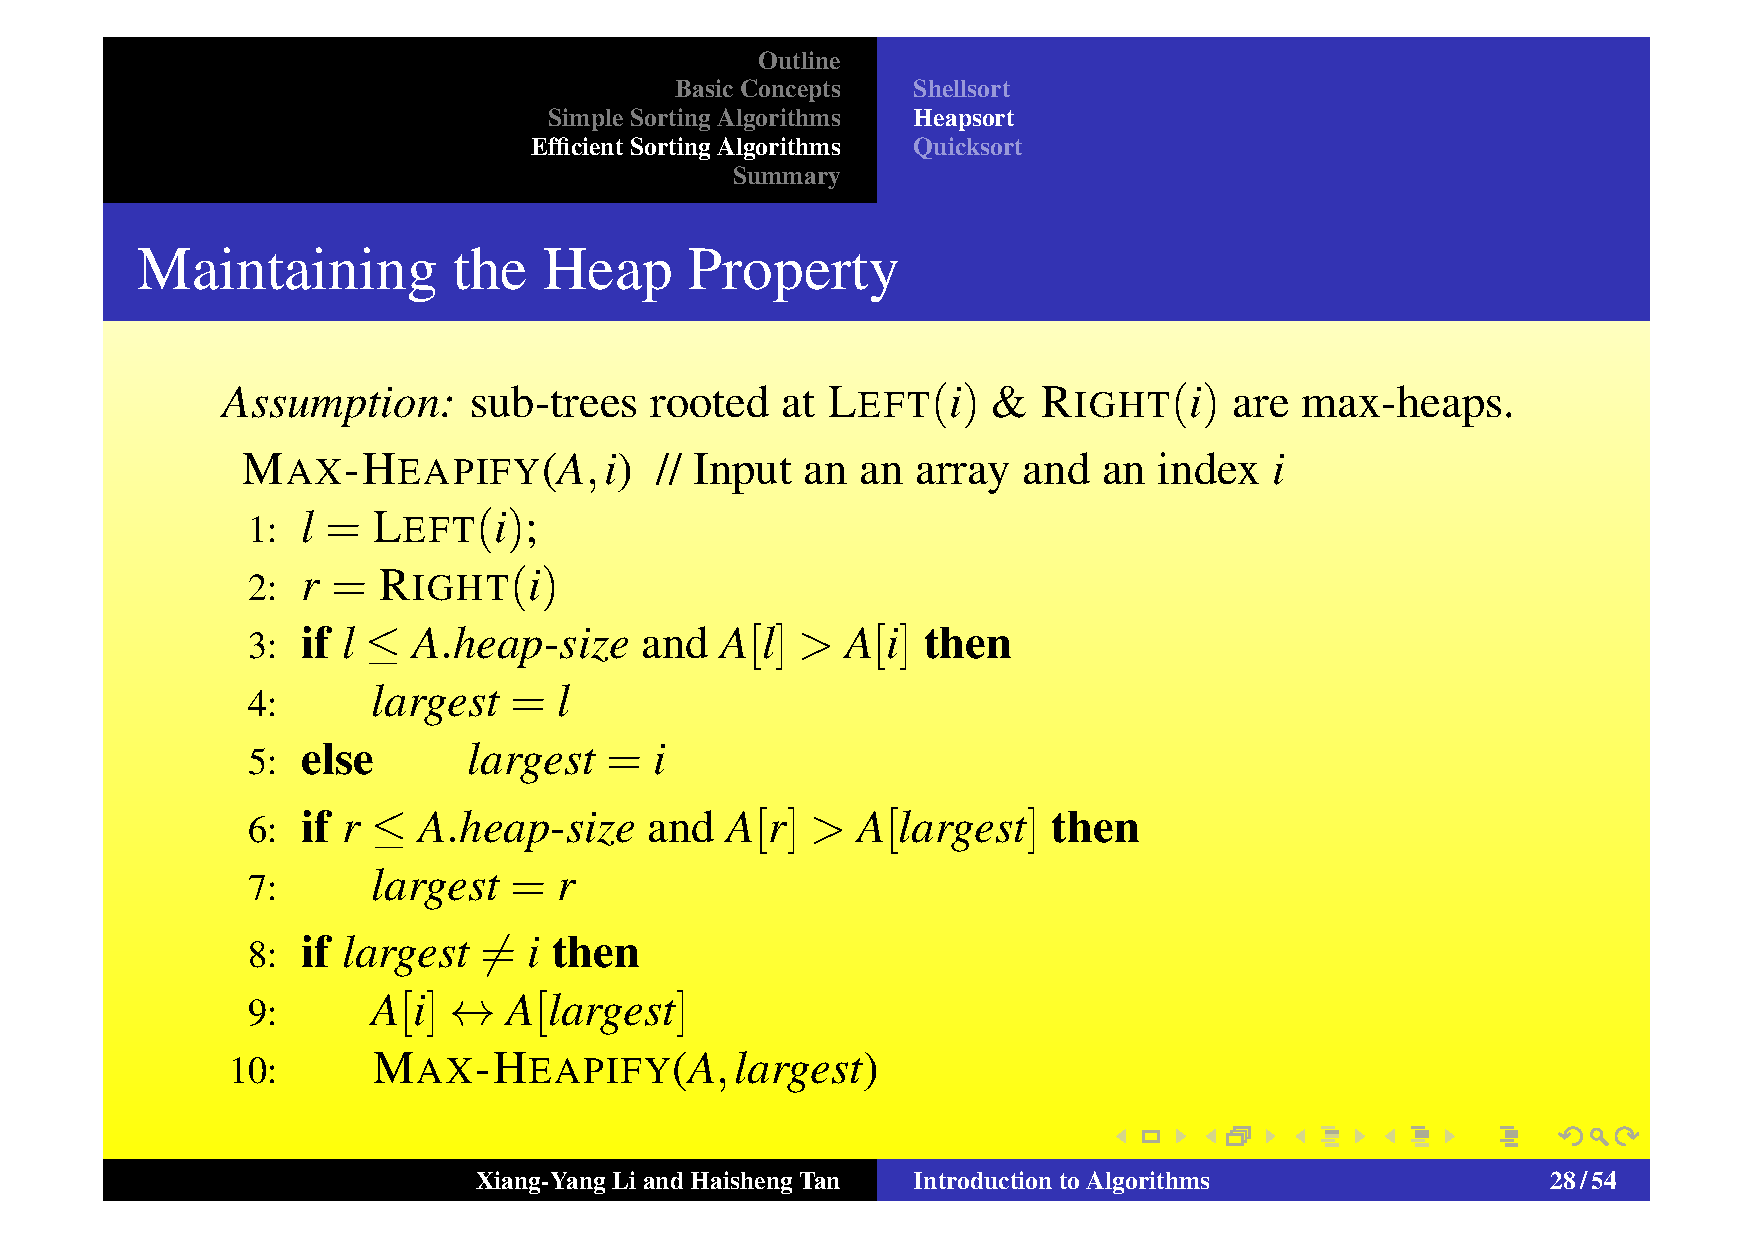
\includegraphics[scale = 0.25]{images/Max_Heapfy.pdf}
			\end{minipage}
		\end{figure}
		时间复杂度:最大堆化$O(\log n)$,建堆$O(n)$;三个总复杂度都是$O(n\log n)$。就地排序但不是稳定排序
		\subsection{优先队列}
		优先队列是一种抽象数据类型,或者说一种需求(如进程调度中的优先级分层调度)。优先队列是一种用来维护由一组元素构成的集合S的数据结构,其中的每一个元素都有一个相关的值,称为关键字key。优先队列中的每个元素都有优先级,而优先级高(或者低)的将会先出队,而优先级相同的则按照其在优先队列中的顺序依次出队。优先队列一般用二叉堆实现(PPT用的最大堆)
	\section{快速排序}
		\textit{很多好的算法都是递归的。}快排({\OldCaption{Quick-Sort}})使用了分治思想。选择一个基准点,作为左右两个子数组的分界标准,然后原问题分解为两个较小的子问题,而由于左数组$A[p..q-1]$的元素均小于$A[q]$,而右数组则相反,故合并过程是平凡的。
		\begin{figure}[h!]
			\centering
			\begin{minipage}{20em}
				\centering
				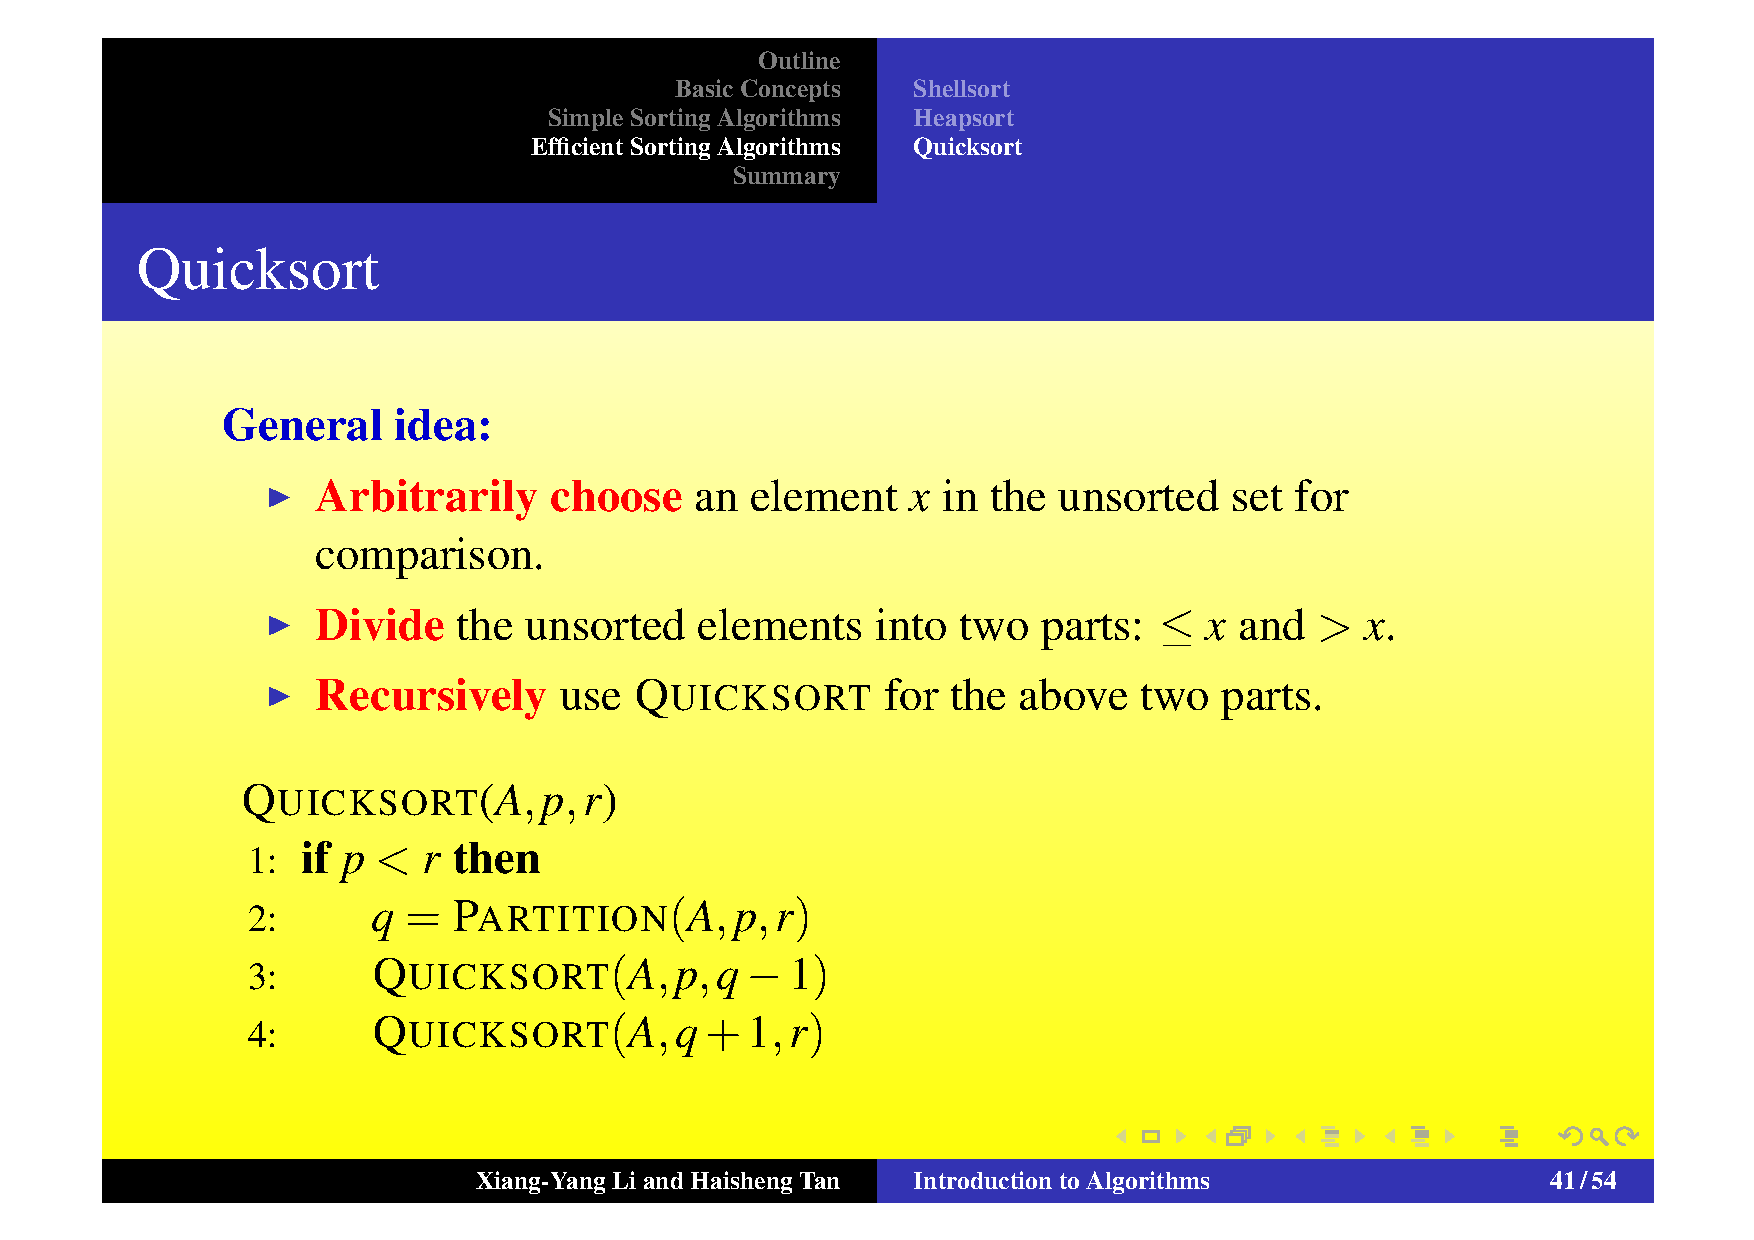
\includegraphics[scale = 0.25]{images/QuickSort.pdf}
			\end{minipage}\quad
			\begin{minipage}{20em}
				\centering
				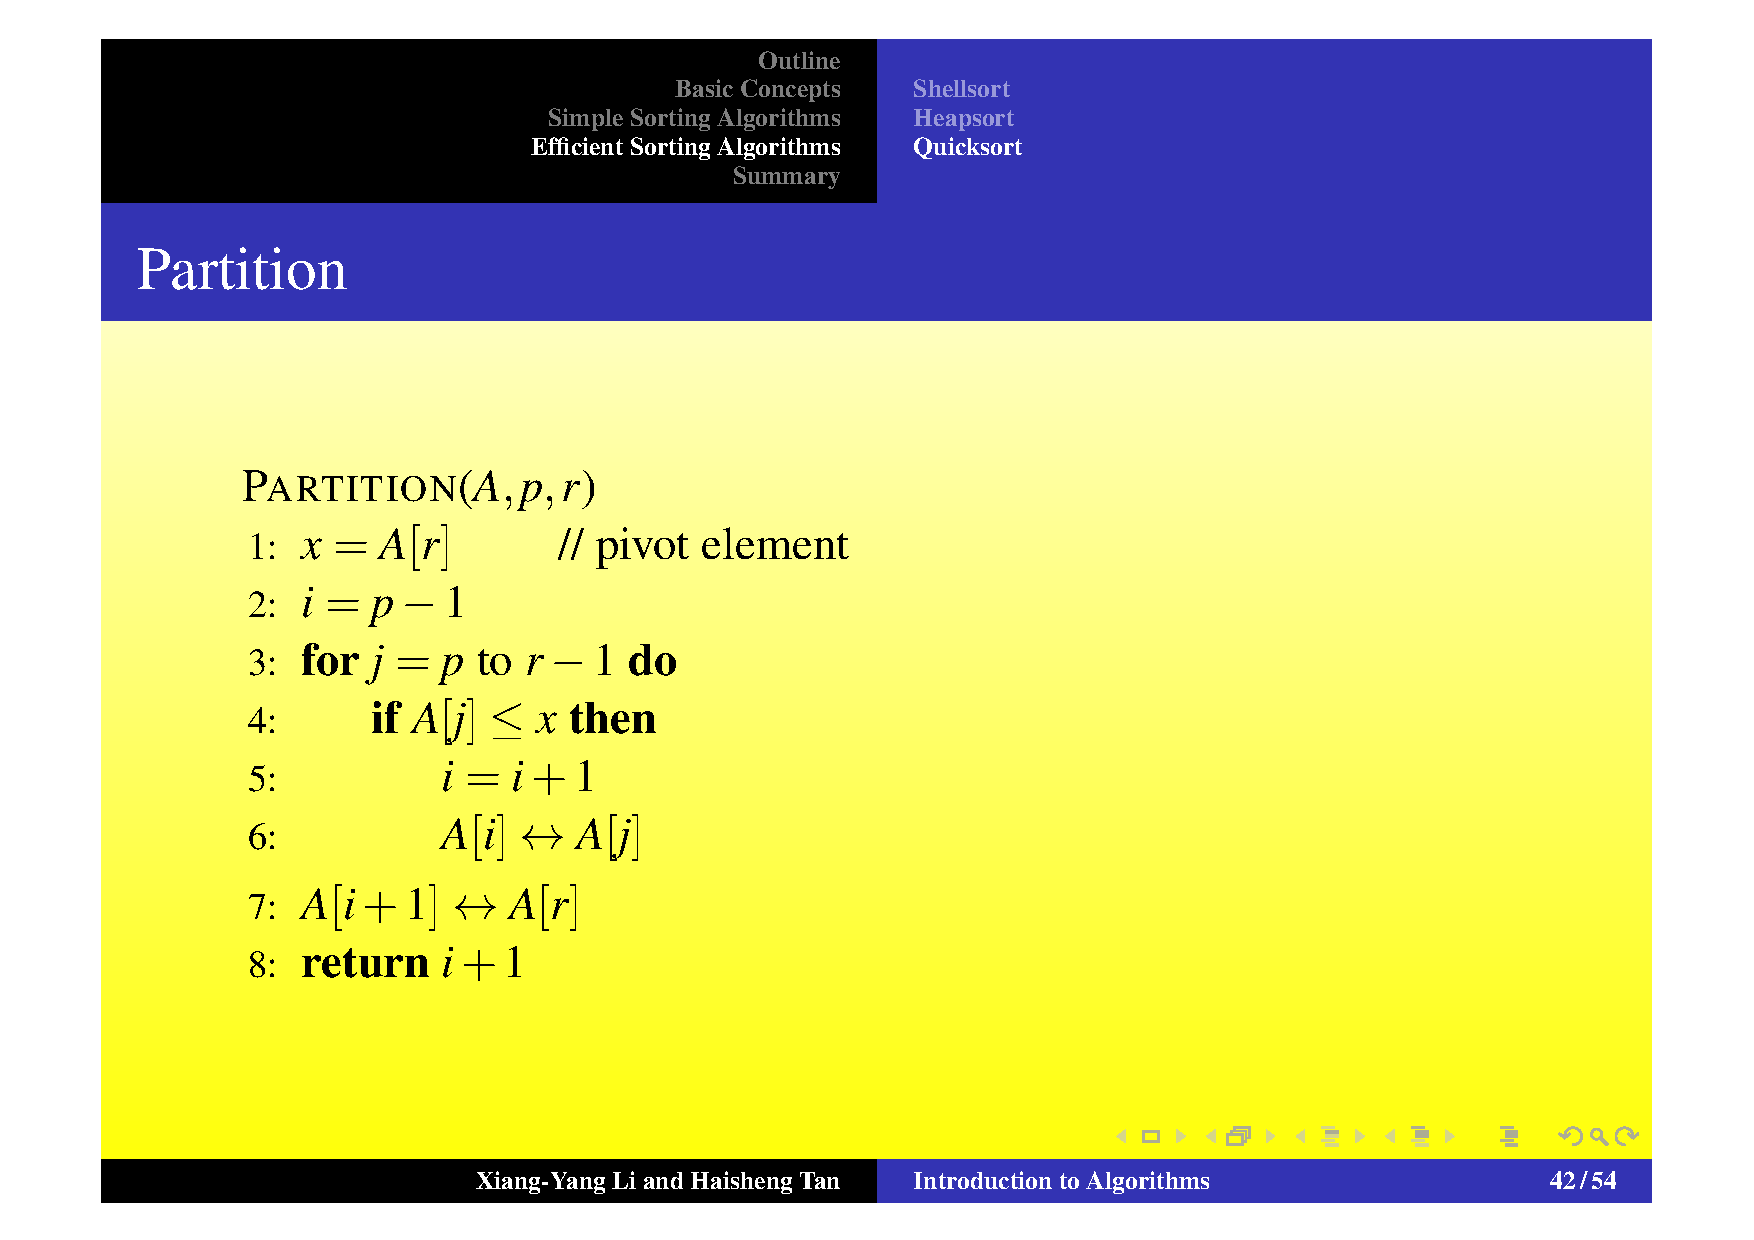
\includegraphics[scale = 0.25]{images/QuickSort_Partition.pdf}
			\end{minipage}
		\end{figure}
		需要引起注意的是,快速排序的时间依赖于划分是否平衡,而平衡与否又依赖于用于划分的元素。如果划分是平衡的,那么性能可以和归并排序一样,如果不是平衡的,那么其性能就接近于插入排序了。如果在算法的每一层递归上,划分都是最大程度不平衡的,那么算法的时间复杂度为$\Theta(n^2)$(这个结论并不依赖于原始数据的整齐程度)。每一次都是平衡的划分,那么他的时间复杂度为$\Theta(n\lg n)$。快排的平均时间复杂度更接近于其最好情况,也是$O(n\lg n)$

	\chapter{线性时间排序}
		所有比较排序算法都有一个共同特点:排出来的顺序只依赖于对于输入元素之间的比较,他们的时间复杂度是$\Omega n$的。比较排序算法可以被抽象地视作(二叉)决策树。\par
		在不同对排序算法之间进行选择对时候,不只是要考虑其时间复杂度,还有一些其他因素。如(characteristics of the implementations)、底层结构(the underlying machine) 以及输入数据(the input data)
	\section{计数排序}
		计数排序({\OldCaption{Counting-Sort}})对整数进行排序,它使用了一个额外的用于计数的数组$C$,其长度取决于待排序数组中数据的范围(等于待排序数组的最大值与最小值的差加上1),这使得计数排序对于数据范围很大的数组,需要大量时间和内存。所以说,计数排序适用于数据量较小的情况。但是,计数排序可以用在基数排序算法中,能够更有效的排序数据范围很大的数组。\par
		计数排序的基本思想是对于数据组中的某一个数据$A$,统计出所有数据中比他小的数据个数为$m$,则他就排在第$m+1$个位置。具体操作是开一个宽度为可能出现的值域宽的统计数组,在遍历原始数据的过程中统计出来所有可能出现的值各自出现了多少次。
		\begin{figure}[h!]
			\centering
			\begin{minipage}{40em}
				\centering
				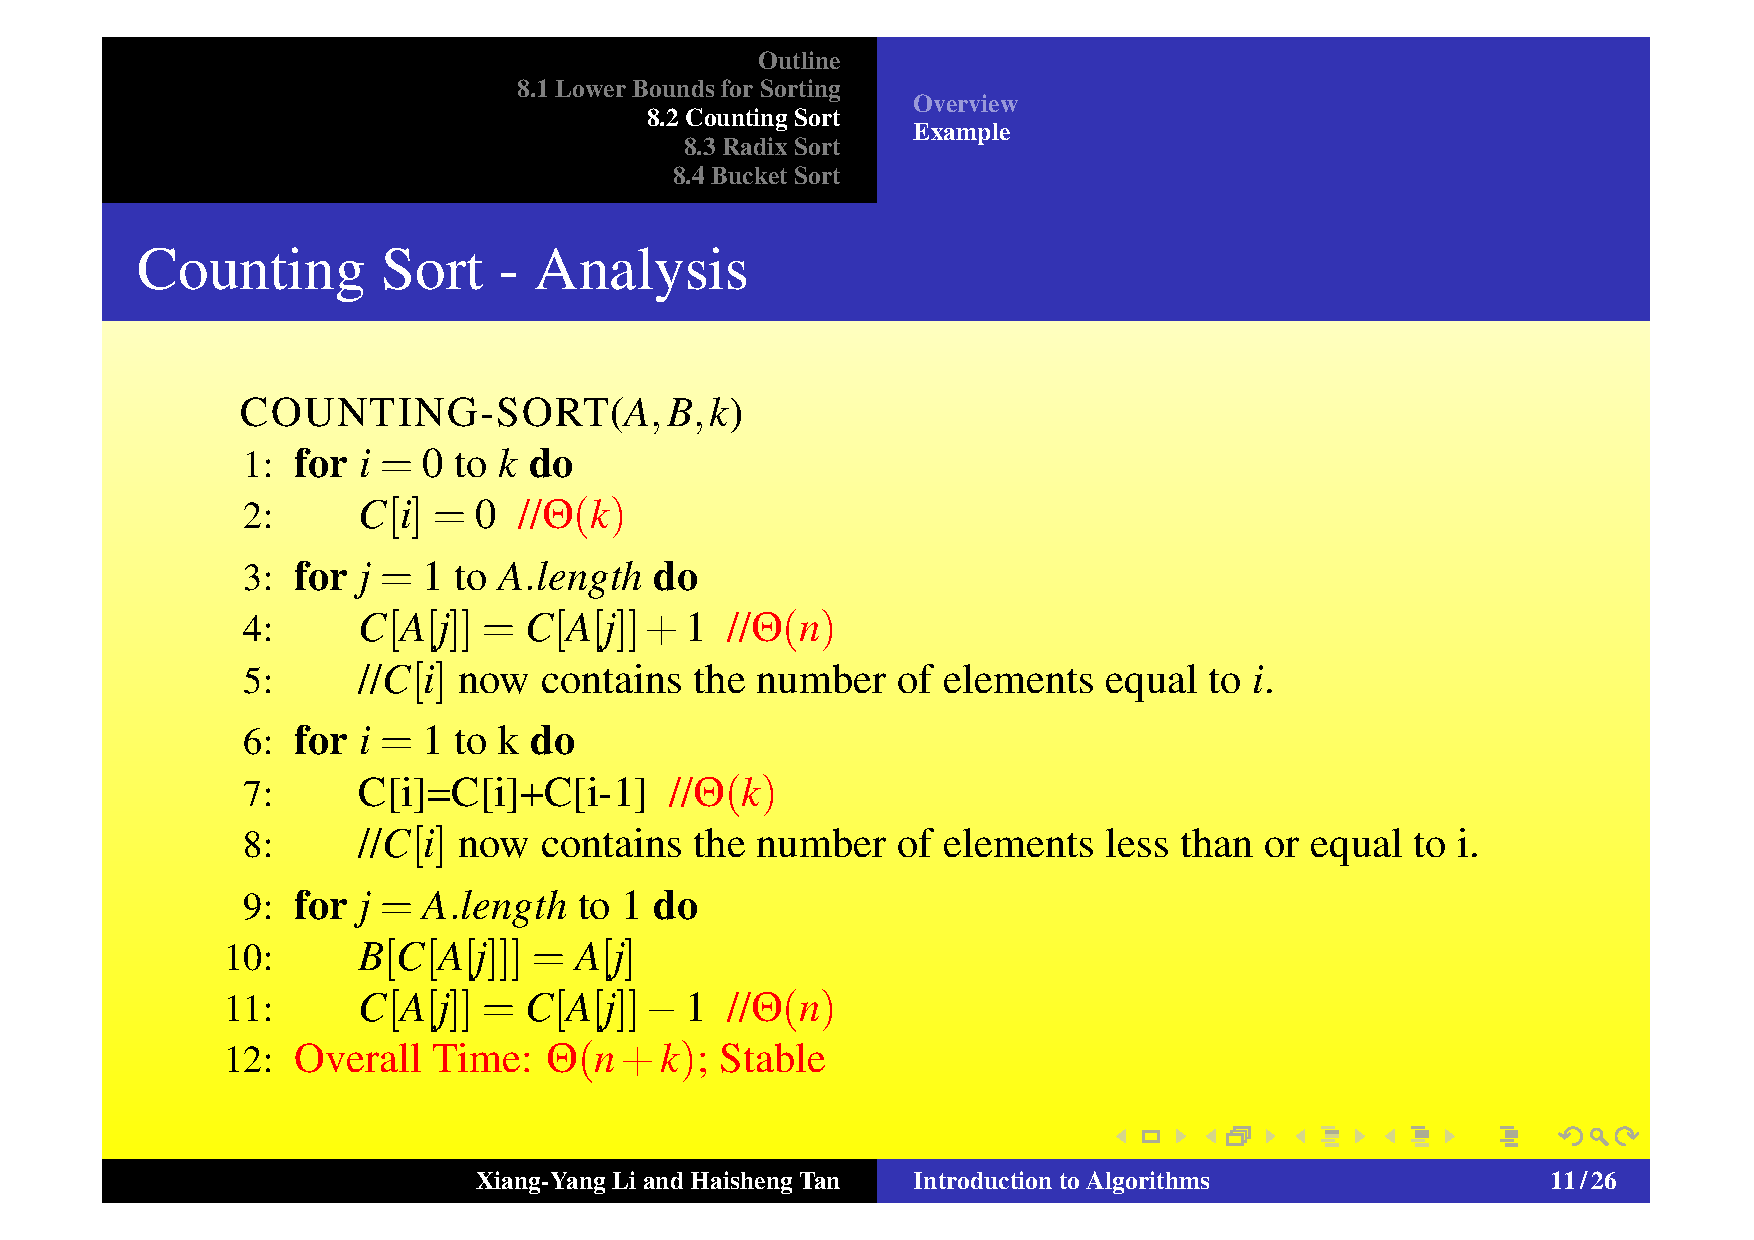
\includegraphics[scale = 0.4]{images/Counting_Sort.pdf}
			\end{minipage}
		\end{figure}
	\section{基数排序}
		基数排序({\OldCaption{Radix-Sort}})是将整数按照位数切割成不同的数字,然后每个位数进行比较。它存在的前提是每一轮排序都是stable的,这样对低位进行的排序保证了在对高位进行排序时,高位相同的数据低位是有序的。收藏一个参考\href{https://www.jianshu.com/p/134a0eed5e3a}{文章}
		\begin{algorithm}
			\caption{{\OldCaption{Radix-Sort}} ($A$,$d$)}
			\KwIn{$A$ is the to-sort array, while $d$ is the 数据位数}
			\For{$i=1$ to $d$}{
				use a stable sort to sort array $A$ on digit $i$
			}
		\end{algorithm}
	\section{桶排序}
		桶排序({\OldCaption{Bucket-Sort}})作用于一组服从在$[0,1)$区间上均匀分布的数据。基本思路是将这个$[0,1)$区间分割成几个等长的小区块,称为“桶”
		\begin{figure}[h!]
			\centering
			\begin{minipage}{20em}
				\centering
				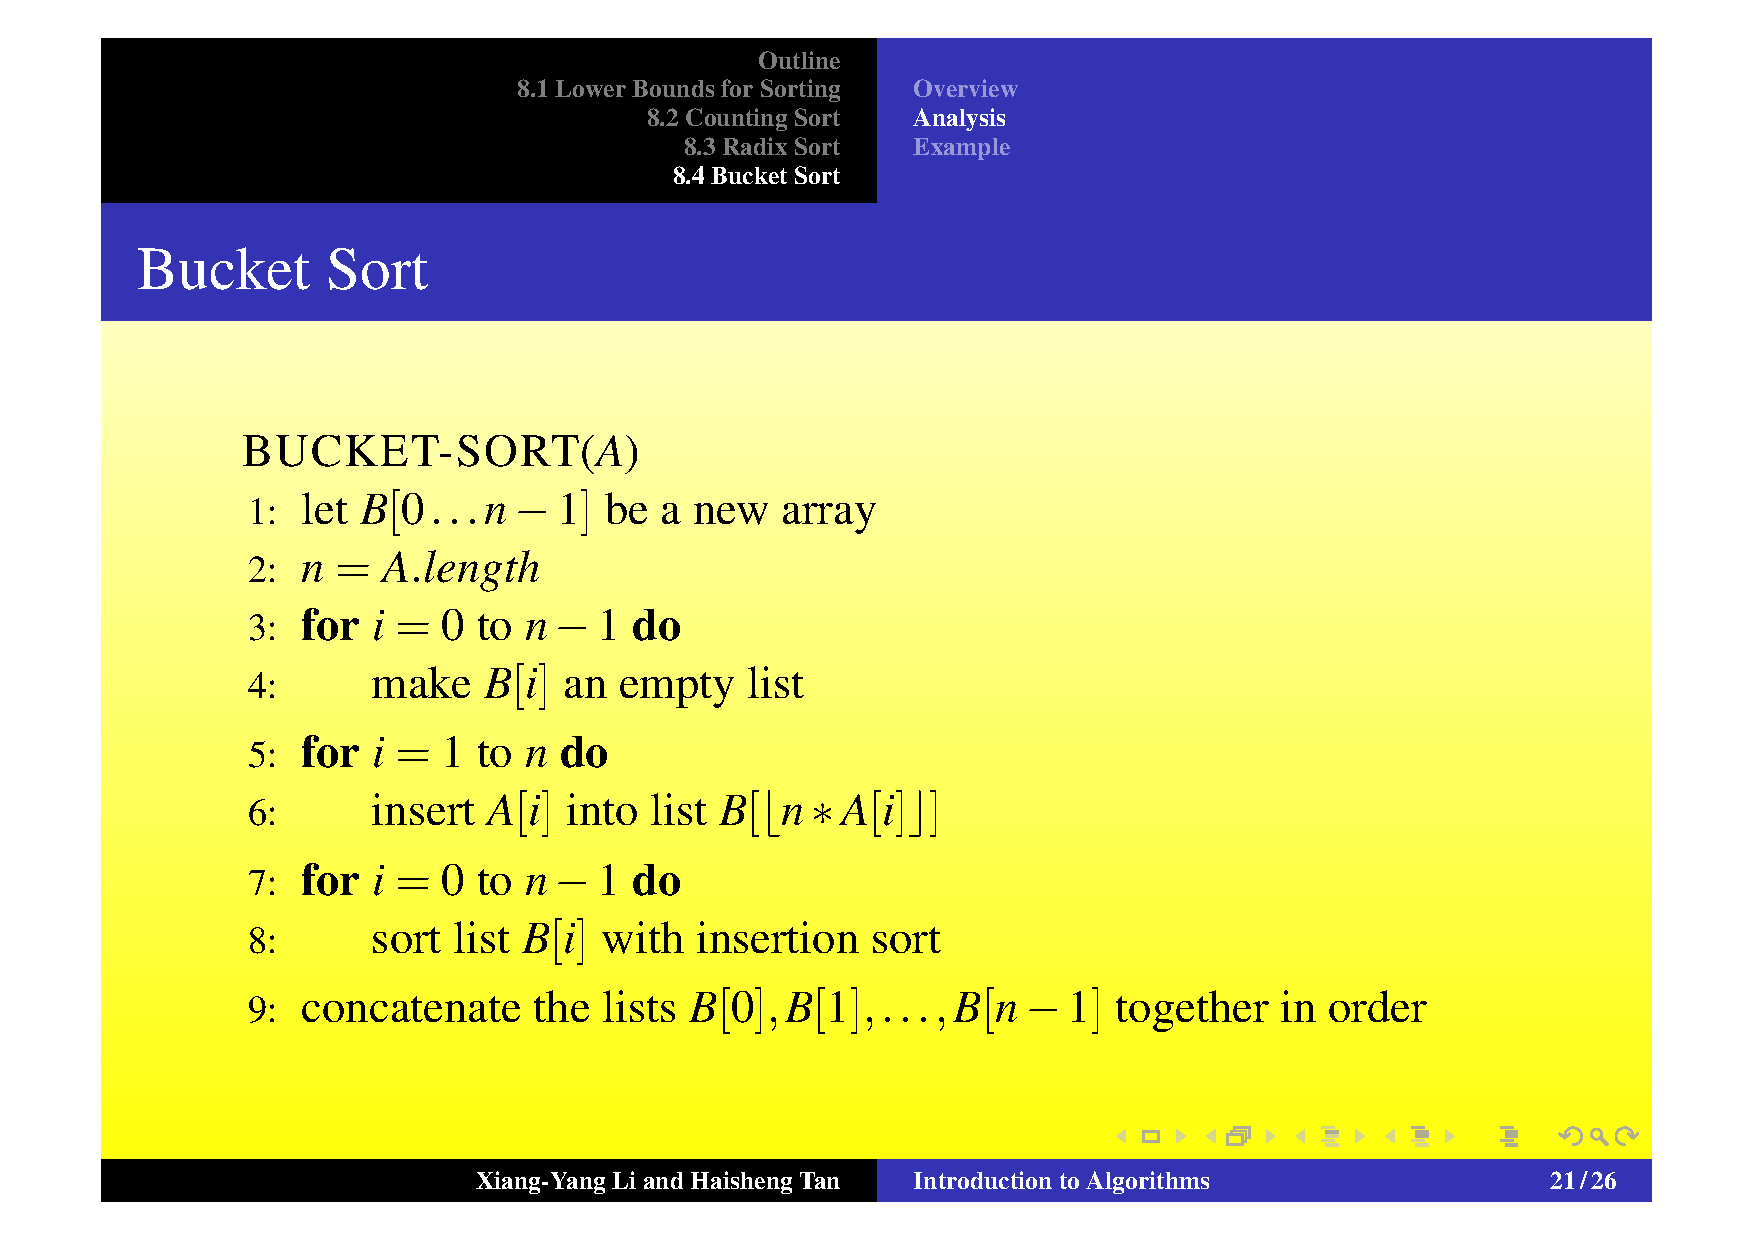
\includegraphics[scale = 0.25]{images/Bucket_Sort_Code.pdf}
			\end{minipage}
			\begin{minipage}{20em}
				\centering
				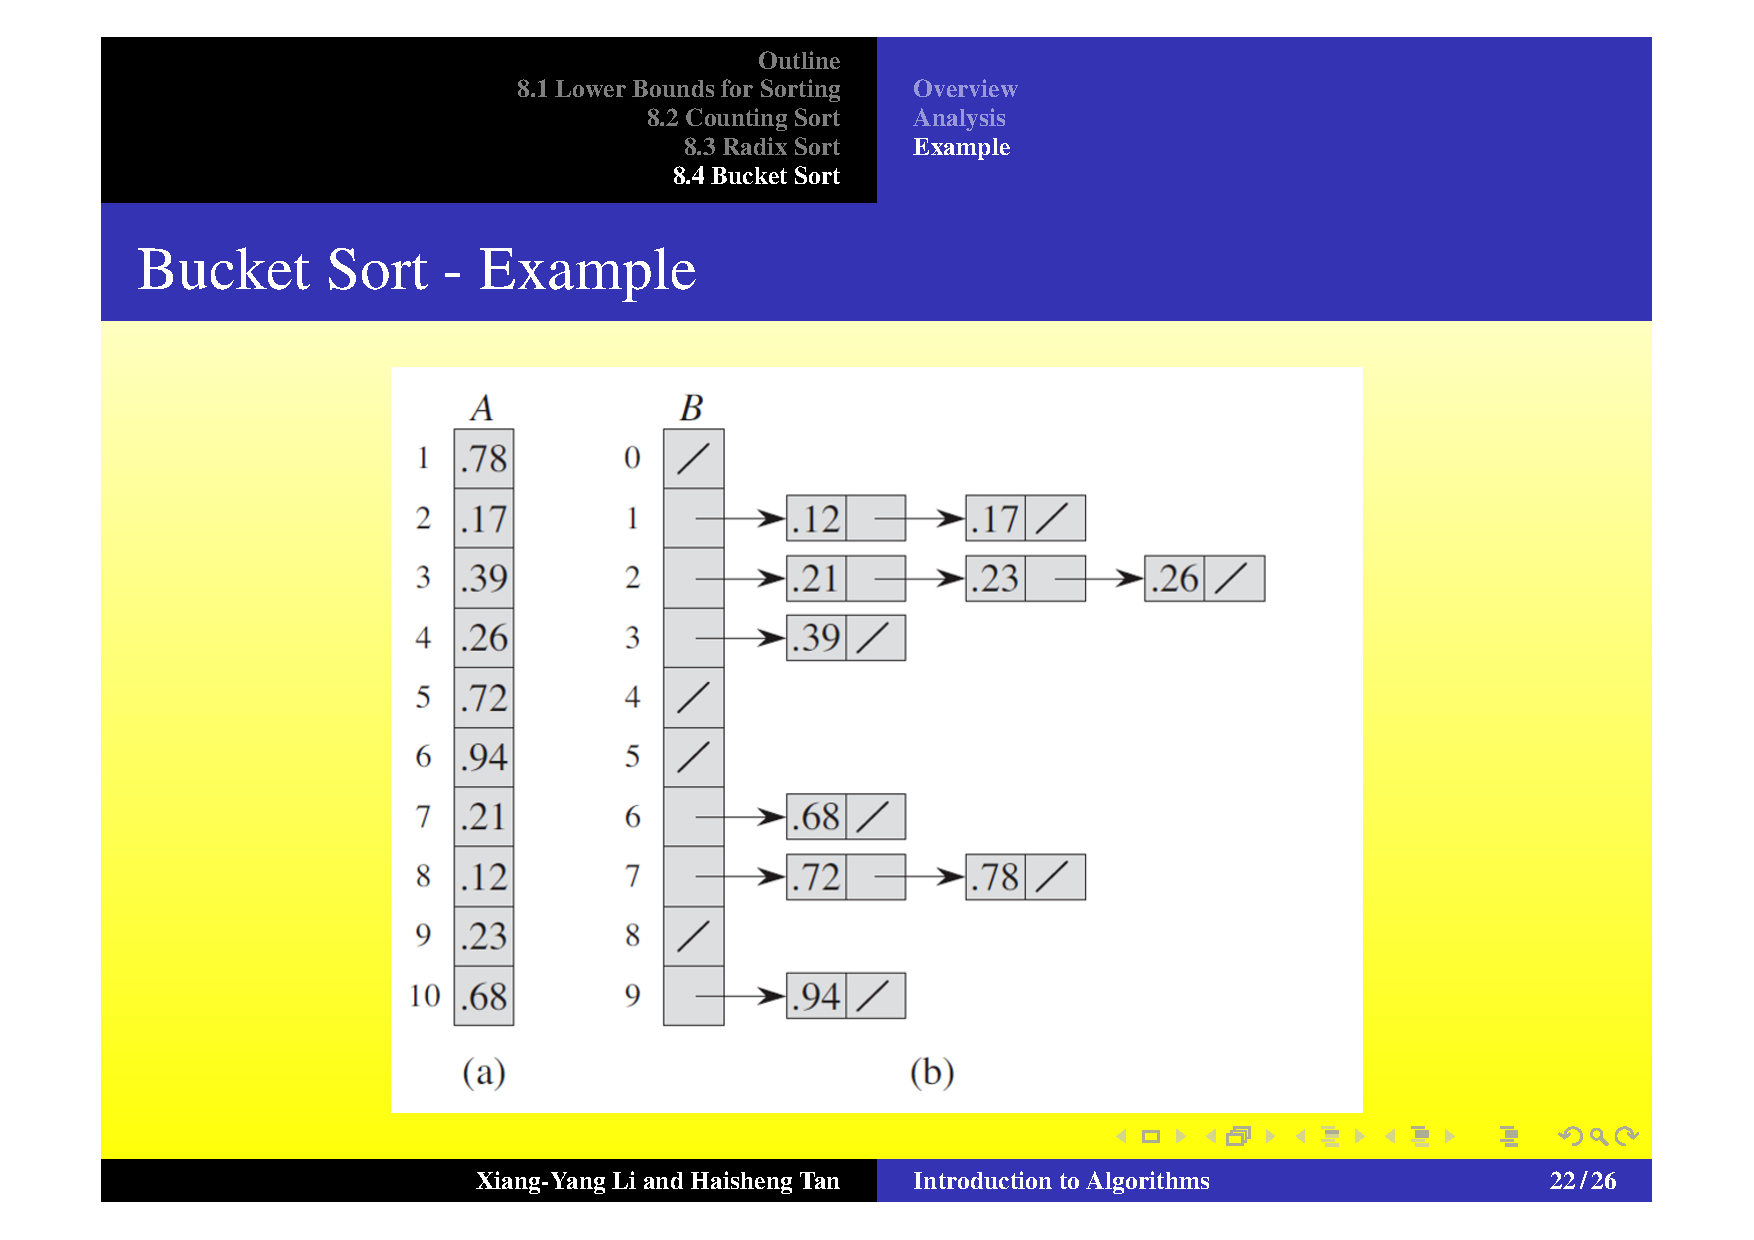
\includegraphics[scale = 0.25]{images/Bucket_Sort_Pic.pdf}
			\end{minipage}
		\end{figure}
		可以证明,桶排序的时间复杂度为$\Theta(n)$。且即使数据不服从均匀分布,桶排序也有可能在线性时间内完成,只要输入数据满足以下的性质:所有桶大小的平方和与总元素数呈线性关系

	\chapter{中位数和顺序统计量}
		本章将讨论一个由n个互异(distinct)元素构成的集合中选择第i个顺序统计量($X_{(i)}$)的问题
	\section{最小值和最大值}
		显然,想要得到一组数据的$\min$和$\max$,最少需要$O(n)$的时间(因为所有数据总要遍历一遍),同时由于比较$n-1$次总能出结果,故最好的次数就是$n-1$。若想要同时找出最小值和最大值,那么就有一种好的算法,只需要最多$3\lceil n/2\rceil$次:对输入的一对元素相互进行比较,然后把较小的与当前最小值比较,较大的与当前最大值进行比较。
	\section{期望为限行时间的选择算法}
		如果想要找到这个集合中的$X_{(k)}$,那么采取一个类似于快排的分治策略:取一个分割点,如果这个点的排序小于k,那么就在高位集合递归,反之在低位集合
\end{document}
